%%
%% Style file "borrowed" from Michel Goemans
%%
\documentclass[11pt]{article}

\usepackage{url,amsmath,amsthm,amsfonts,amssymb}
\usepackage{pgf}

\def\ceil#1{\lceil #1 \rceil}
\def\floor#1{\lfloor #1 \rfloor}
\def\ang#1{\langle #1 \rangle}

\newtheorem{definition}{Definition}
\newtheorem{remark}{Remark}
\newtheorem{theorem}{Theorem}
\newtheorem{lemma}[theorem]{Lemma}
\newtheorem{corollary}[theorem]{Corollary}
\newtheorem{proposition}[theorem]{Proposition}
\newtheorem{claim}[theorem]{Claim}
\newtheorem{observation}{Observation}

\newcommand{\R}{{\mathbb R}}
\newcommand{\Var}{\hbox{Var}}
\newcommand{\Z}{{\mathbb Z}}
\newcommand{\Q}{{\mathbb Q}}
\newcommand{\C}{{\mathbb C}}
\newcommand{\N}{{\mathbb N}}

\newlength{\toppush}
\setlength{\toppush}{2\headheight}
\addtolength{\toppush}{\headsep}

\newcommand{\htitle}[2]{\noindent\vspace*{-\toppush}\newline\parbox{6.5in}
 {\large Addis Ababa University, Amist Kilo \hfill #1\newline
\hspace*{\fill}{\bf Algorithms and Programming for High Schoolers} \hspace*{\fill} \newline
\mbox{}\hrulefill\mbox{}}\vspace*{1ex}\mbox{}\newline
\begin{center}{\Large\bf #2}\end{center}}

\newcommand{\handout}[3]{\thispagestyle{empty}
 \markboth{ #2}{ #2}
 \pagestyle{myheadings}\htitle{\protect\ref{#1}}{#2}{#3}}

\setlength{\oddsidemargin}{0pt}
\setlength{\evensidemargin}{0pt}
\setlength{\textwidth}{6.5in}
\setlength{\topmargin}{0in}
\setlength{\textheight}{8.5in}

\newcommand{\eps}{\varepsilon}
\newcommand{\sq}[1]{\langle#1\rangle}

\begin{document}

\htitle{August 2, 2016}{Lecture 12}

\paragraph{\Large Graphs:}

A {\em graph} is a pair $(V,E)$, where $V$ is called the set of {\em
  vertices} and $E$ is called the set of {\em edges}.  
Edges are pairs of vertices and represent some form of connection
between two vertices.  Many pieces of data can be thought of in a
graph representation.  For example, we can think of the Facebook
graph: there would be one vertex for each person on Facebook, and an
edge exists between two people if they are friends.  Such graphs are
called {\em undirected}, meaning that the the connection an edge
represents between two vertices is mutual: if you and I form an edge
on Facebook then I am your friend, and you are also my friend.  The
Twitter graph on the other hand is not
undirected.  Suppose an edge (x,y) means that x follows y on Twitter.
Then John may follow Bob, but Bob may not follow John, which means the
graph would have the edge (John, Bob) but not (Bob, John).  Graphs in
which an edge (x,y) are treated as being different from (y,x), such as
the Twitter graph, are called {\em directed}.

\medskip
\textbf{Graph examples:}
\begin{itemize}
\item Social networks (Facebook, MySpace, Twitter, Google+,
  $\ldots$). People are vertices, and edges mean
  friendship/following/etc.
\item The web graph. Web pages are vertices, and an edge (x,y) means
  page x has a link to page y.
\item Road networks. Street intersections are vertices, and an edge
  (x,y) means a person at intersection x can reach intersection y by a
  segment of road.
\item Airport networks. Airports are vertices, and an edge (x,y) means
  there's a direct flight from x to y.
\item Family trees. People are vertices, and an edge (x,y) means x
  is one of the parents of y.
\end{itemize}

Today we discuss algorithms to answer a few basic questions about
graphs.  Before doing that though, we have to discuss how the graph is
given as input to the computer. The two most popular ways of
specifying a graph are via an {\em adjacency matrix} or an {\em
  adjacency list}.  

\begin{figure}[!!h]
\begin{center}
\scalebox{0.5}{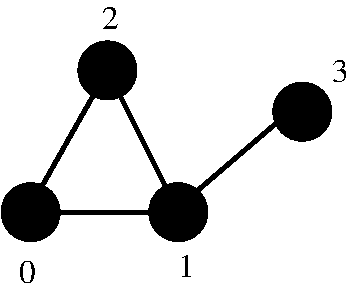
\includegraphics{graph}}
\end{center}
\caption{Example undirected graph.}
\end{figure}

Suppose the graph has $n$ vertices, which we label
from $0$ to $n-1$.  Then, an adjacency matrix is simply a
\texttt{list} $A$ of $n$ \texttt{list}s, where each \texttt{list} is
of size $n$.  The entry $A[i][j]$ is \texttt{True} if the edge $(i,j)$
exists in
the graph, and otherwise it is \texttt{False}.  For example, we could
represent
the graph in Figure 1 as follows:
\begin{align*}
 \mathrm{A} &= [ [\texttt{False}, \texttt{True}, \texttt{True},
\texttt{False}], [\texttt{True}, \texttt{False}, \texttt{True},
\texttt{True}], \\
&\hspace*{.25in}[\texttt{True}, \texttt{True}, \texttt{False},
\texttt{False}], [\texttt{False}, \texttt{True}, \texttt{False},
\texttt{False}] ] .
\end{align*}

In adjacency list representation, we have a variable $A$ which is a
\texttt{list} of $n$ \texttt{list}s.  The $i$th list contains a list
of all vertices $j$ such that $(i,j)$ is an edge in the graph.  So,
we could represent Figure 1 in adjacency list representation as
follows:
$$ A = [ [1, 2], [0, 2, 3], [0, 1], [1] ] .$$

Each representation has its own advantages, and the situation should
dictate which one is best to use.  For example, the adjacency matrix
representation always requires $\Theta(n^2)$ memory, whereas the
adjacency list representation can take much less memory if the graph
has few edges.  Meanwhile, the adjacency matrix representation can
tell you whether $i$ has an edge to $j$ in $O(1)$ time (just look at
$A[i][j]$), whereas it could take $\Omega(n)$ time in the adjacency
list representation if $i$ has many edges, since you might have to
scan the entire $i$th list.

\paragraph{Graph exploration:}

Now we will cover algorithms to answer some of the most basic questions
about graphs.  These are questions such as:

\begin{itemize}
\item \textbf{Connectedness:} Given vertices $i,j$, are they {\em
    connected}?  That is, is there a {\em
    path} from $i$ to $j$?  A path is just a sequence of edges that
  share endpoints.  In other words, can I start at $i$, follow some
  sequence of edges, then end up at $j$?
\item \textbf{Connected components:} A connected a component of an
  undirected graph is a set of vertices that are all
  connected to each
  other via paths, and are not connected to anything else.
\item \textbf{Shortest path:} Given vertices $i,j$, what's the
  shortest number of edges you have to cross to get from $i$ to $j$?
\end{itemize}

We will be able to answer the questions above using search algorithms
known as {\em depth-first search} and {\em bread-first search}.
First, we will need to discuss two data structures known as the {\em
  stack} and the {\em queue}.

\begin{itemize}
\item A {\em \textbf{stack}} is a collection of data items that supports two
  operations: \texttt{push(x)} and \texttt{pop()}.  \texttt{push}(x)
  puts the item x at the top of the stack, and \texttt{pop}() returns
  the item at the top of the stack then deletes it from the stack.
  You should picture a stack of papers: when you want the next paper
  you just take it off the top (\texttt{pop()}), and when you add to
  the pile you just put it on the top (\texttt{push()}).
\item A {\em \textbf{queue}} is a collection of data items that
  also supports \texttt{push(x)} and \texttt{pop()}, but they work in
  different ways.  Now you should imagine the data items sitting in a
  line, like at a movie theater.  When a new person enters a line, he
  enters the back, and the next person to be taken from the line is
  the one at the front.  Programming \textbf{queue}s work in the same
  way: new data items are pushed onto the back of the queue, and
  \texttt{pop()} returns the item at the front of the queue then
  deletes it from the queue.
\end{itemize}

Stacks support what is known as LIFO (last-in-first-out) since the
last item to enter the stack is the first one to be popped out.
Meanwhile, queues are FIFO (first-in-first-out).

Stacks and queues are easily implemented in Python using the
\texttt{list}, though for efficiency reasons it's recommended that you
use the deque data structure built into Python.

\begin{verbatim}
# Using a stack
stack = []
stack.append(5) # a push operation; same as stack += [5]
stack.append(6)
y = stack.pop() # stack is now [5], and y is 6
y = stack.pop() # stack is now [], and y is 5
\end{verbatim}

\begin{verbatim}
# Using a queue
from collections import deque
queue = deque()
queue.append(5) # a push operation; same as queue += [5]
queue.append(6)
y = queue.popleft() # queue is now [6], and y is 5
y = queue.popleft() # queue is now [], and y is 6
\end{verbatim}

We are now ready to cover the two graph-exploration algorithms
depth-first search and breadth-first search.  Below are the
algorithms assuming the graph is given in adjacency list
representation.  

\paragraph{Depth-first search}

\begin{verbatim}
def visit(x, stack, visited):
    visited[x] = True
    stack += [x] # push x

# do a depth-first search (dfs) from vertex v, where A is the
# adjacency list of the graph
def dfs(A, v):
    visited = [False]*len(A)
    stack = []
    visit(v, stack, visited)
    while len(stack) > 0:
        x = stack.pop()
        for y in A[x]:
            if not visited[y]:
                visit(y, stack, visited)
\end{verbatim}

A recursive implementation would have the same effect since recursion
is implemented using a stack:

\begin{verbatim}
def visit(x, visited):
    visited[x] = True
    for y in A[x]:
        if not visited[y]:
            visit(y, visited)

# do a depth-first search (dfs) from vertex v, where A is the
# adjacency list of the graph
def dfs(A, v):
    visited = [False]*len(A)
    visit(v, visited)
\end{verbatim}

\paragraph{Breadth-first search}

\begin{verbatim}
from collections import deque

def visit(x, queue, visited):
    visited[x] = True
    queue += [x] # push x

# do a breadth-first search (bfs) from vertex v, where A is the
# adjacency list of the graph
def bfs(A, v):
    visited = [False]*len(A)
    queue = deque()
    visit(v, queue, visited)
    while len(queue) > 0:
        x = queue.popleft()
        for y in A[x]:
            if not visited[y]:
                visit(y, queue, visited)
\end{verbatim}

The dfs and bfs algorithms for graph exploration are quite similar,
except that the former uses a stack and the latter uses a queue.  This
has an effect on the order in which vertices are visited.  Consider
the two following pictures, each of the same graph, but one visited in
dfs order and the other in bfs order.

\begin{figure}[!!h]
\begin{center}
\begin{tabular}{c|c}
\scalebox{0.5}{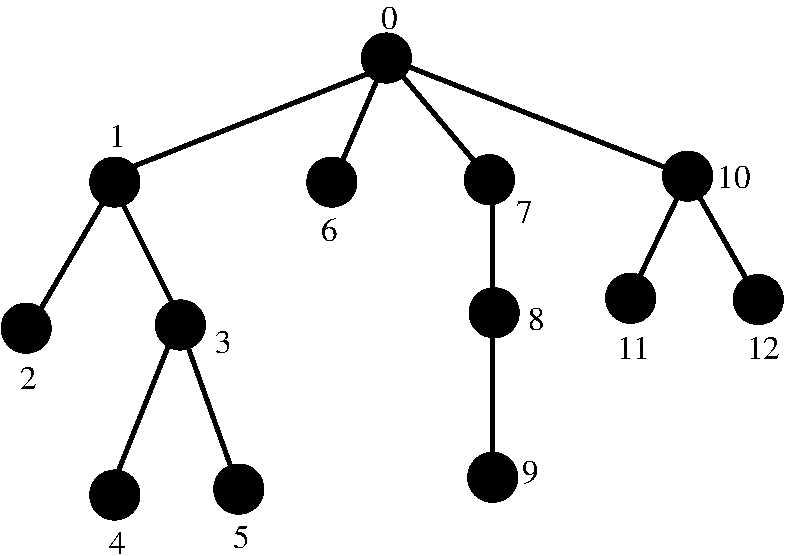
\includegraphics{dfs}} &
\scalebox{0.5}{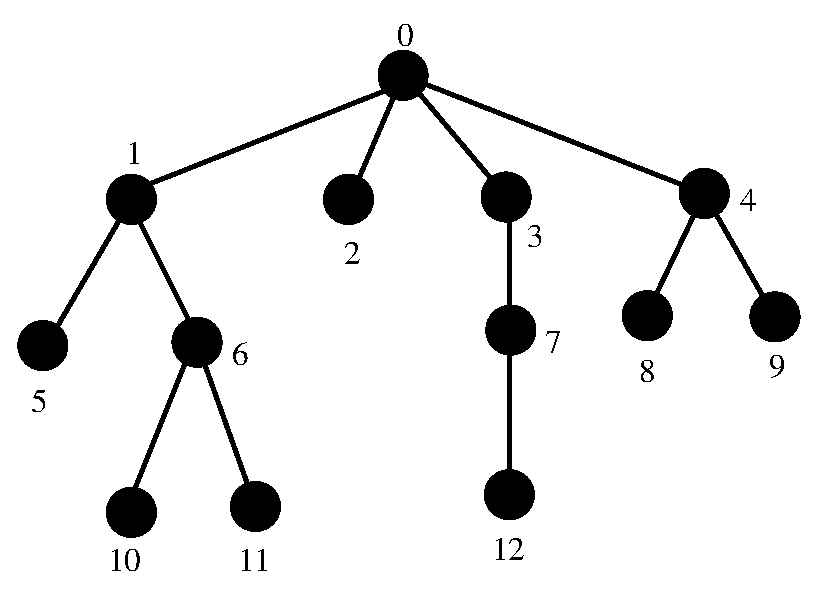
\includegraphics{bfs}}
\end{tabular}
\end{center}
\caption{The same graph, being visited in dfs order on the left, and
  in bfs order on the right.  The numbers represent the order in which
the vertices are visited (0 is visited first, and 12 
last).}
\end{figure}

In effect, bfs order visits all vertices which are distance 1 away
from the start first, then all vertices which are distance 2 away,
etc.  Meanwhile, dfs keeps following edges until it hits a dead end,
then it backtracks until the last time it wasn't at a dead end and
follows the other branch(es).

Given dfs and bfs, answering some of the questions above is simple.
To test whether a vertex $i$ is connected to a vertex $j$ via some
path, we just dfs or bfs from $i$ and check whether we ever
\texttt{pop} $j$ off the stack in the \texttt{while} loop.  To find
connected components, we can dfs or bfs from every vertex in a graph
and see which other vertices get visited (and once a vertex is
visited, we have found its connected component, so we don't have to
initiate a dfs or bfs from it).  To find a shortest path from $i$ to
$j$, we can use bfs since it visits vertices in order of their
distance from the starting point.

\end{document}
